\documentclass[11pt]{beamer}
\usepackage[utf8]{inputenc}
\usepackage[croatian]{babel}
\usepackage[T1]{fontenc}
\usepackage{amsmath}
\usepackage{amsfonts}
\usepackage{amssymb}
\usepackage{graphicx}
\usepackage{fixmath}
\usepackage{booktabs}
\usepackage{caption}
%\usecolortheme[snowy]{owl}
\usetheme{metropolis}

\usefonttheme[onlymath]{serif}

\newcommand{\q}{\left}
\newcommand{\w}{\right}

\newcommand{\matr}[1]{\mathbold{#1}}
\newcommand{\prob}[1]{\operatorname{\mathbf{P} \q(#1\w)}}
\renewcommand{\alert}{\textbf}

\setlength{\jot}{2ex}

\begin{document}
  \author{Lovre Mrčela, Andro Merćep, Stjepan Begušić, and Zvonko Kostanjčar}
  \title{Portfolio Optimization Using Preference Relation Based on Statistical Arbitrage}
  \institute{\textbf{University of Zagreb} \\
			 Faculty of Electrical Engineering and Computing \\
			 Laboratory for Financial Risk Assessment \\
             Zagreb, Croatia}
  \date{18/10/2017}
  \setbeamertemplate{navigation symbols}{}

  \begin{frame}[plain]
  \maketitle
  \end{frame}

%  \begin{frame}{Contents}
%    \setbeamertemplate{section in toc}[sections numbered]
%    \tableofcontents[hideallsubsections]
%  \end{frame}
%  
  \section{Introduction}
  \begin{frame}
    \frametitle{Introduction}
    \begin{itemize}
    \item \alert{portfolio optimization}
    \item enhancement of present methods of \alert{statistical arbitrage}
    \item modeling \emph{asset interactions} using \alert{preference flow graph}
    \end{itemize}
  \end{frame}

%  \begin{frame}
%    \frametitle{Teorem o nearbitraži}
%    \begin{theorem}
%      Ako je u trenutku 0 vrijednost portfelja $V\q(0\w) = 0$, tada je u nearbitražnim okolnostima vjerojatnost $\prob{V\q(t\w) > 0} = 0$ za $t > 0$.
%    \end{theorem}
%  \end{frame}

%  \begin{frame}
%    \frametitle{Koeficijent obrtaja}
%    \begin{itemize}
%      \item \emph{mjera promjenljivosti} portfelja
%      \item u rasponu $\q[0, 2\w]$
%      \item portfelj s $N$ vrijednosnica $\matr{\alpha} = \begin{bmatrix} \alpha_1 & \alpha_2 & \cdots & \alpha_N \end{bmatrix}$
%      \item \alert{koeficijent obrtaja} $\eta^{(t)}$:
%      \begin{equation*}
%        \eta^{(t)} = \sum_{i=1}^{N} \q \lvert \alpha_i^{(t)} - \alpha_i^{(t-1)} \w \rvert
%      \end{equation*}
%      \item \emph{veći koeficijent obrtaja --- veći troškovi trgovanja}
%    \end{itemize}
%  \end{frame}
  
  \section{Concepts and methods}
  \begin{frame}
    \frametitle{Statistical arbitrage}
    \only<1>{
    Outline of statistical arbitrage methods:
    \begin{enumerate}
      \item \alert{identifying} pairs of assets whose prices behave \emph{similarly} during the past period,
      \item \alert{choosing} pairs which demonstrate a \emph{statistically significant deviation} at the present moment,
      \item \alert{assuming} \emph{short} position in one asset of a pair and \emph{long} position in other asset of pair for each pair,
      \item \alert{closing} positions once deviation is no longer present.
    \end{enumerate}}
    \only<2>{
     \begin{figure}
       \centering
       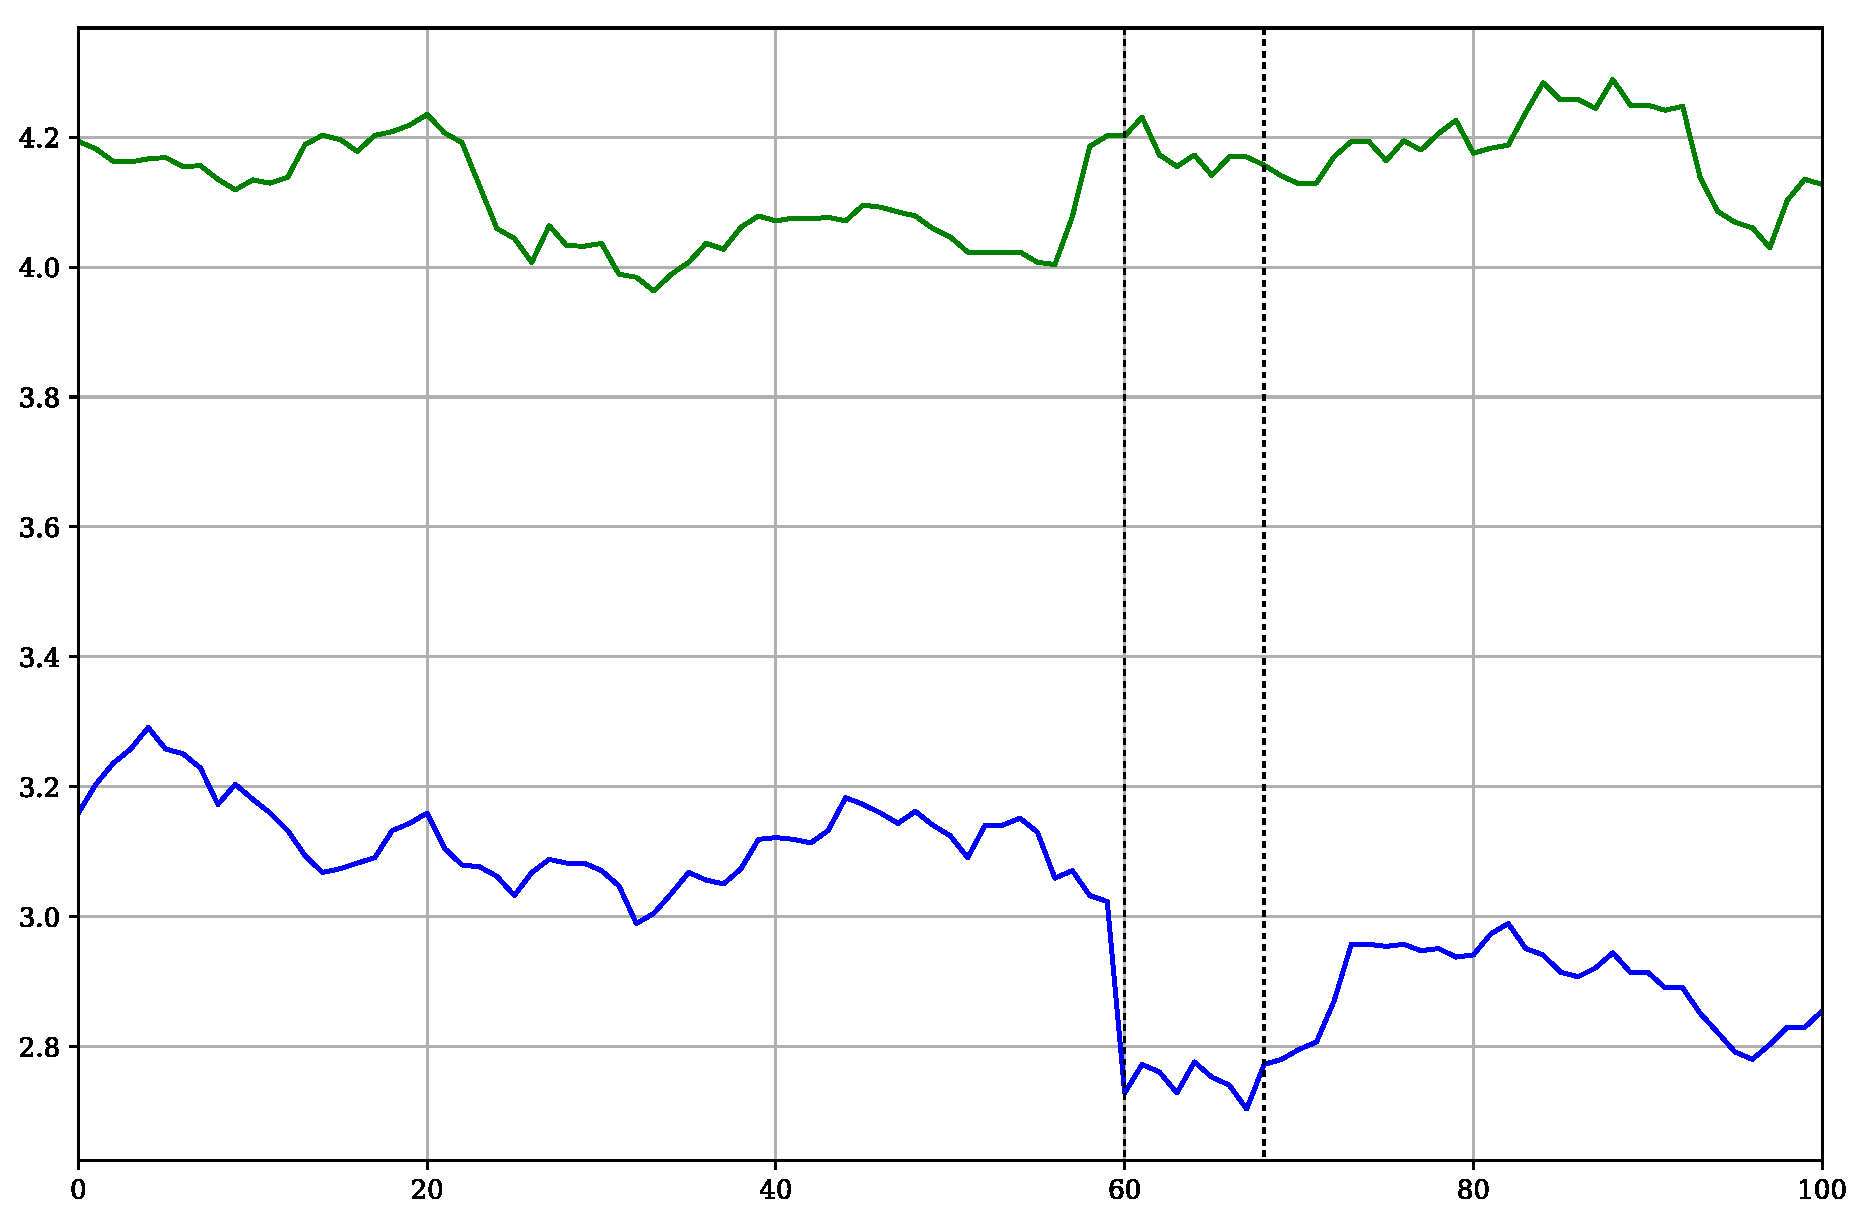
\includegraphics[width=\textwidth]{graphics/trading-signal.pdf}
       \caption*{Log prices of a pair of assets.}
     \end{figure}}
%     \only<3>{
%       \begin{figure}
%         \centering
%         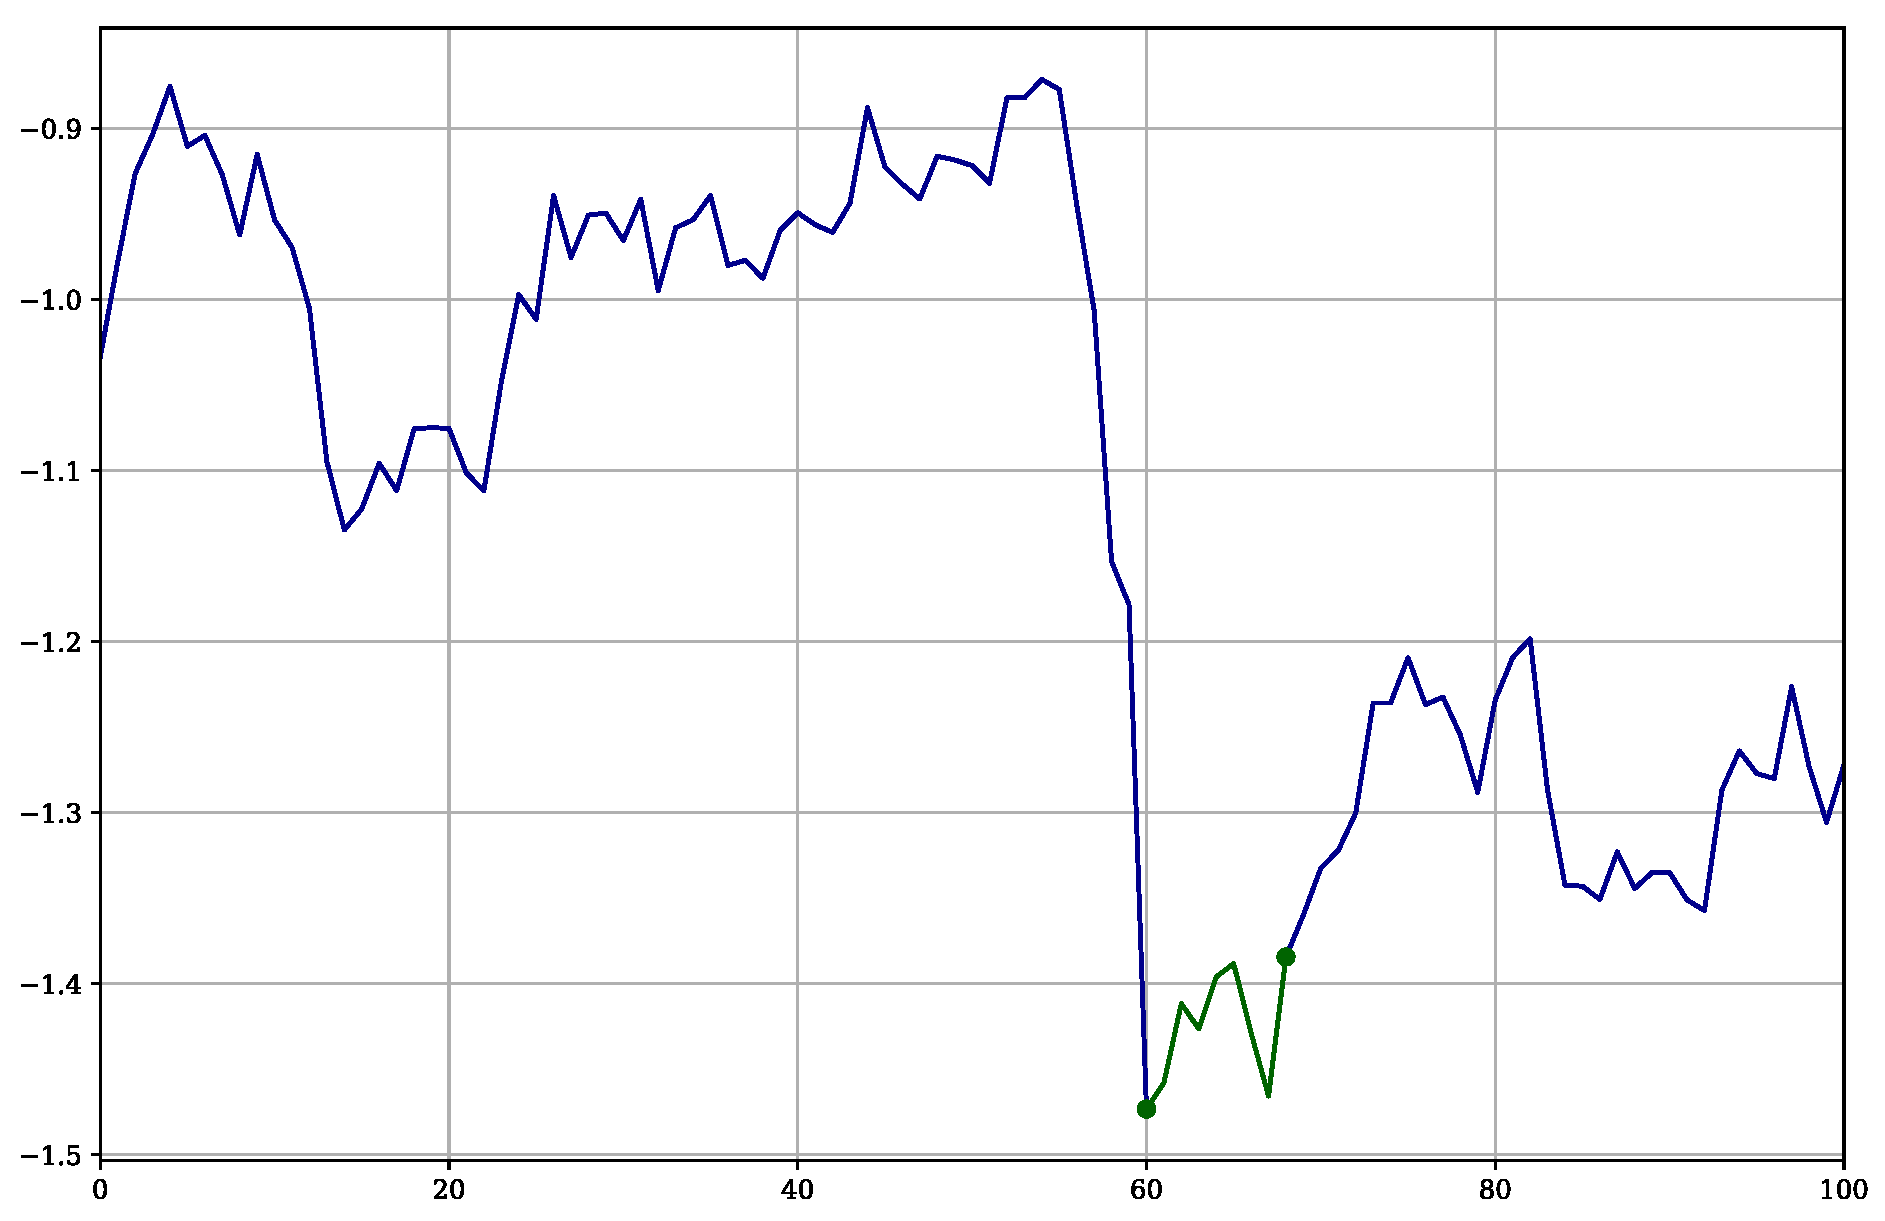
\includegraphics[width=\textwidth]{graphics/trading-diffs.pdf}
%         \caption*{Log price difference of the same two assets.}
%     \end{figure}}
  \end{frame}

%  \begin{frame}
%    \frametitle{Trading signal}
%    \only<1>{
%      \begin{gather*}
%      c_{i,j} \text{ --- log price difference of assets } i \text{ and } j \\
%      m_{i,j}^{\q(t\w)} = \frac{1}{T}\sum_{\tau = t - T}^{t - 1} c_{i,j}^{(\tau)} \\
%      d_{i,j}^{\q(t\w)} = \sqrt{\frac{1}{T - 1}\sum_{\tau=t - T}^{t - 1} \q(c_{i,j}^{(\tau)} - m_{i,j}^{\q(t\w)} \w)^2} \\
%      \Gamma_{X, Y}^{(t)} = \frac{c_{X,Y}^{
%          \q(t\w)} - m_{X,Y}^{\q(t\w)}}{d_{X,Y}^{\q(t\w)}}
%      \end{gather*}
%    }
%    \only<2>{
%    \begin{figure}
%      \centering
%      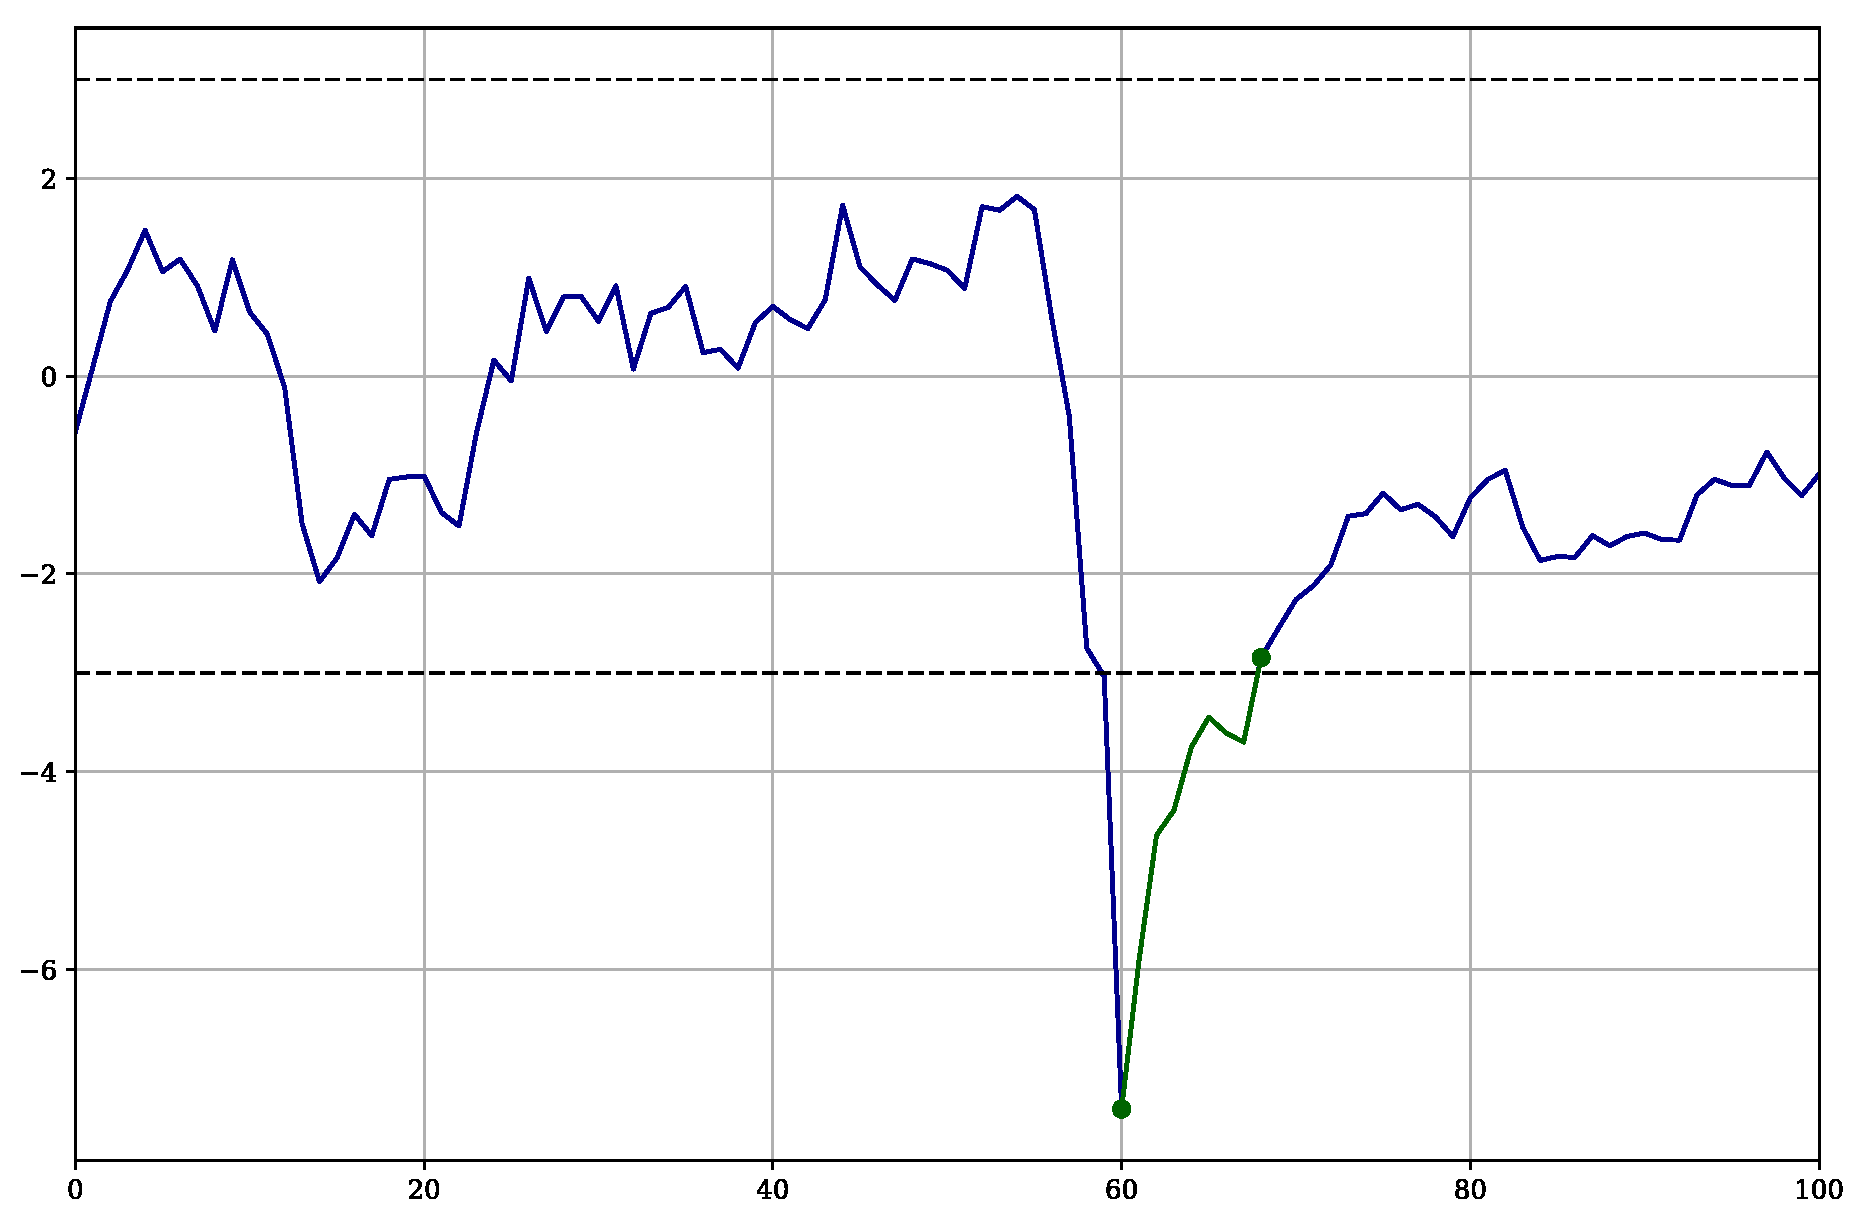
\includegraphics[width=\textwidth]{graphics/trading-prices.pdf}
%      \caption*{Trading signal obtained from previous two assets.}
%    \end{figure}}
%  \end{frame}

  \begin{frame}
    \frametitle{Cons of statistical arbitrage method}
    \begin{itemize}
      \item low precision (in the sense of predicting price rise/fall): in most simulations \textbf{less than 50\%}
%      \item trading always done in pairs (\emph{short} and \emph{long} positions); requires possibility of \alert{short position} on the market
      \item doesn't expand well to more pairs
      \item frequent changes of the portfolio result in \alert{significant transaction costs}
    \end{itemize}
  \end{frame}

  \section{Algorithm}
  \begin{frame}
    \frametitle{Preference relation}
    \begin{itemize}
      \item \textbf{binary relation:} $a \succ b$ %($a$ is \emph{more preferred} than $b$)
      \item \emph{incomparability} of entities: $a \sim b$ %($a$ \emph{is not comparable} to $b$)
      \item a more \emph{natural} way of comparing entities
      \item it is \emph{irreflexive}, \emph{asymmetric}, \emph{transitive}, and \emph{transitive in incomparability} 
    \end{itemize}
  \end{frame}

  \begin{frame}
    \frametitle{Preference flow graph}
    \only<1>{
    \begin{itemize}
      \item \emph{preference relation} does not define \emph{ordering} of goods, no \emph{intensities} of preference are specified
      \item \alert{preference flow graph} introduces \emph{intensities} of preference, and models \emph{asset interaction}
      \item utility structure for obtaining explicit ordering of assets
      \item may be intrinsically \alert{inconsistent}
    \end{itemize}}
    \only<2>{
      \begin{figure}
        \centering
        \begin{minipage}{0.45\textwidth}
          \centering
          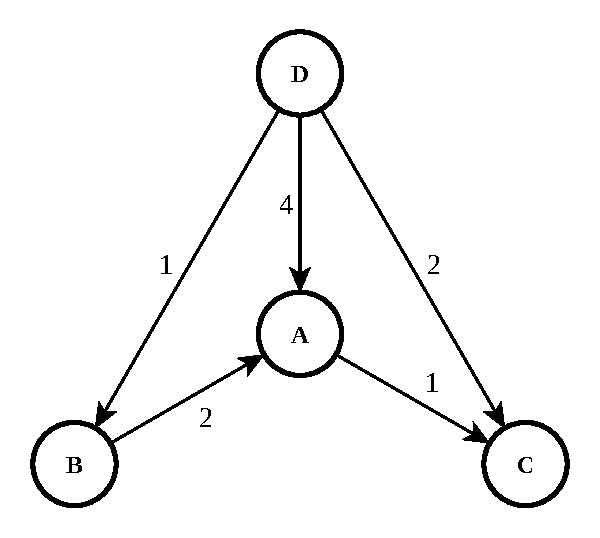
\includegraphics[width=0.808\textwidth]{graphics/graph-eg-1.pdf}
          \caption*{Inconsistent graph.}
        \end{minipage}
        \hfill
        \begin{minipage}{0.45\textwidth}
          \centering
          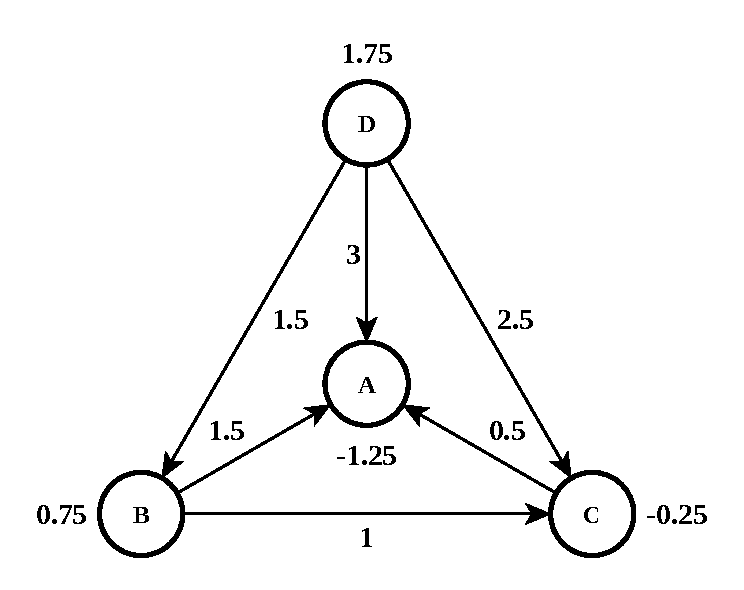
\includegraphics[width=\textwidth]{graphics/graph-eg-2.pdf}
          \caption*{Consistent graph.}
        \end{minipage}
      \end{figure}}
  \end{frame}

  \begin{frame}
    \frametitle{Potential method}
    \only<1>{
    \begin{itemize}
%      \item \alert{preference flow graph} too doesn't define \emph{ordering} of assets
      \item \alert{potential method} introduces \emph{ordering} of goods, and gives a \alert{consistency measure} of the graph
      \item \emph{consistency measure} describes \emph{confidence} in a trading decision
    \end{itemize}}
    \only<2>{
      \begin{figure}
        \centering
        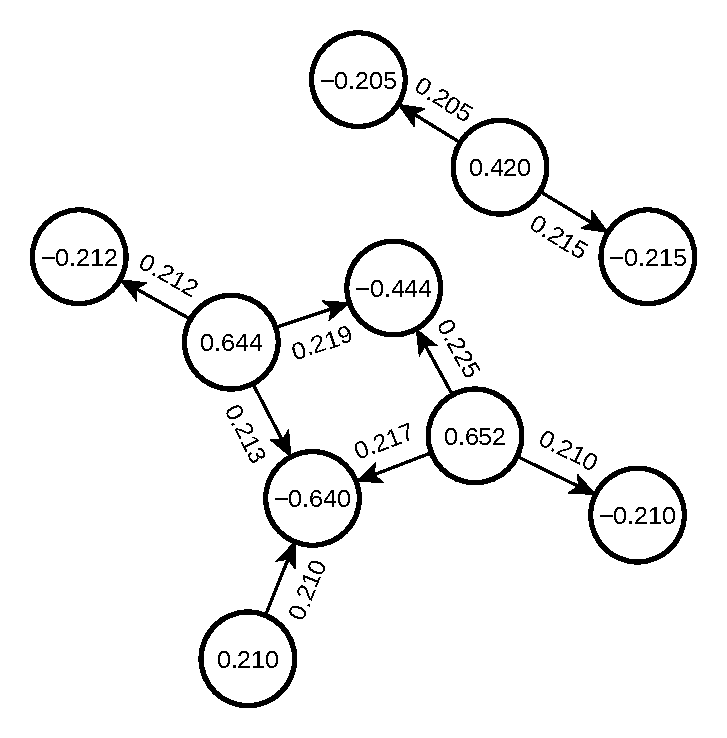
\includegraphics[width=0.6\textwidth]{graphics/pref-flow-graph.pdf}
        \caption*{Results of applying the \emph{potential method} on a \emph{preference flow graph}.}
      \end{figure}}
  \end{frame}

  \begin{frame}
    \frametitle{Summary of trading algorithm}
    \begin{enumerate}
      \item obtain preference flows among the assets using \emph{statistical arbitrage method}
      \item construct \emph{preference flow graph}, then apply the \emph{potential method} to impose ordering by \emph{preference}
      \item take \textbf{long} position in assets with the \textbf{highest} preference, and  \textbf{short} position in assets with the \textbf{lowest} preference (if short position is allowed)
    \end{enumerate}
  \end{frame}

  \section{Results}
%  \begin{frame}
%    \frametitle{Implementacija}
%    \begin{itemize}
%      \item \alert{\textit{Python}} (\emph{NumPy}, \emph{pandas}, \emph{SciPy}, \emph{Matplotlib})
%      \item \alert{\textit{Jupyter} bilježnica}
%      \item \emph{open source} alati
%      \item metoda statističke arbitraže i metoda potencijala
%      \item skripte za simuliranje trgovanja
%    \end{itemize}
%  \end{frame}

  \begin{frame}
    \frametitle{Simulation results --- subset from S\&P 500}
    \only<1>{
    \begin{figure}
      \centering
      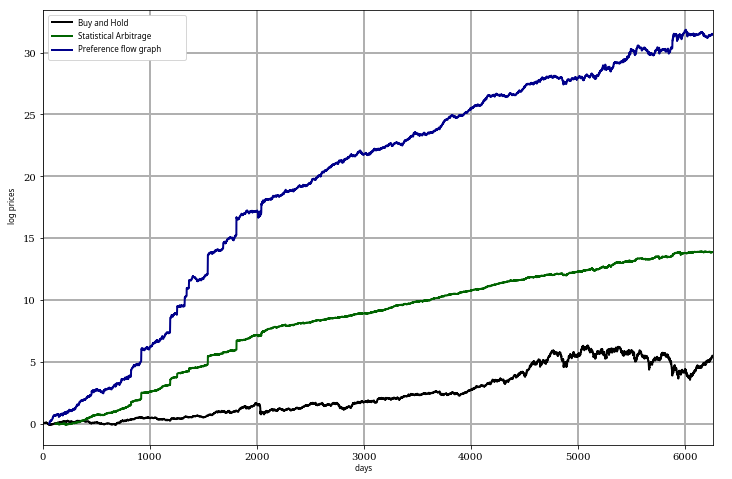
\includegraphics[width=\textwidth]{graphics/result1.png}
      \caption*{Simulation results on a subset of 203 assets from S\&P 500 index.}
    \end{figure}}
    \only<2>{
      \begin{table}
        \centering
        \caption*{Simulation results on a subset of 203 assets from S\&P 500 index.}
        \resizebox{\textwidth}{!}{\begin{tabular}{lrrr}
          \toprule
          \textbf{Method} & Buy \& Hold & Statistical arbitrage & Preference flow \\
          \midrule
          \textbf{Annual return} & 0.07622 & 0.63033 & \textbf{1.28000} \\
          \textbf{Volatility} & \textbf{0.15069} & 0.33532 & 0.78373 \\
          \textbf{Sharpe ratio} & 0.50582 & \textbf{1.87981} & 1.63322 \\
          \textbf{Average turnover rate} & / & 1.473211 & \textbf{0.55112} \\
          \midrule
          \textbf{Net profit with 0.10\% transaction costs} & 5.49572 & --2.74051 & 24.66204 \\
          \bottomrule
        \end{tabular}}
      \end{table}}
\end{frame}

%  \begin{frame}
%    \frametitle{Simulation results --- S\&P 500}
%    \only<1>{
%      \begin{figure}
%        \centering
%        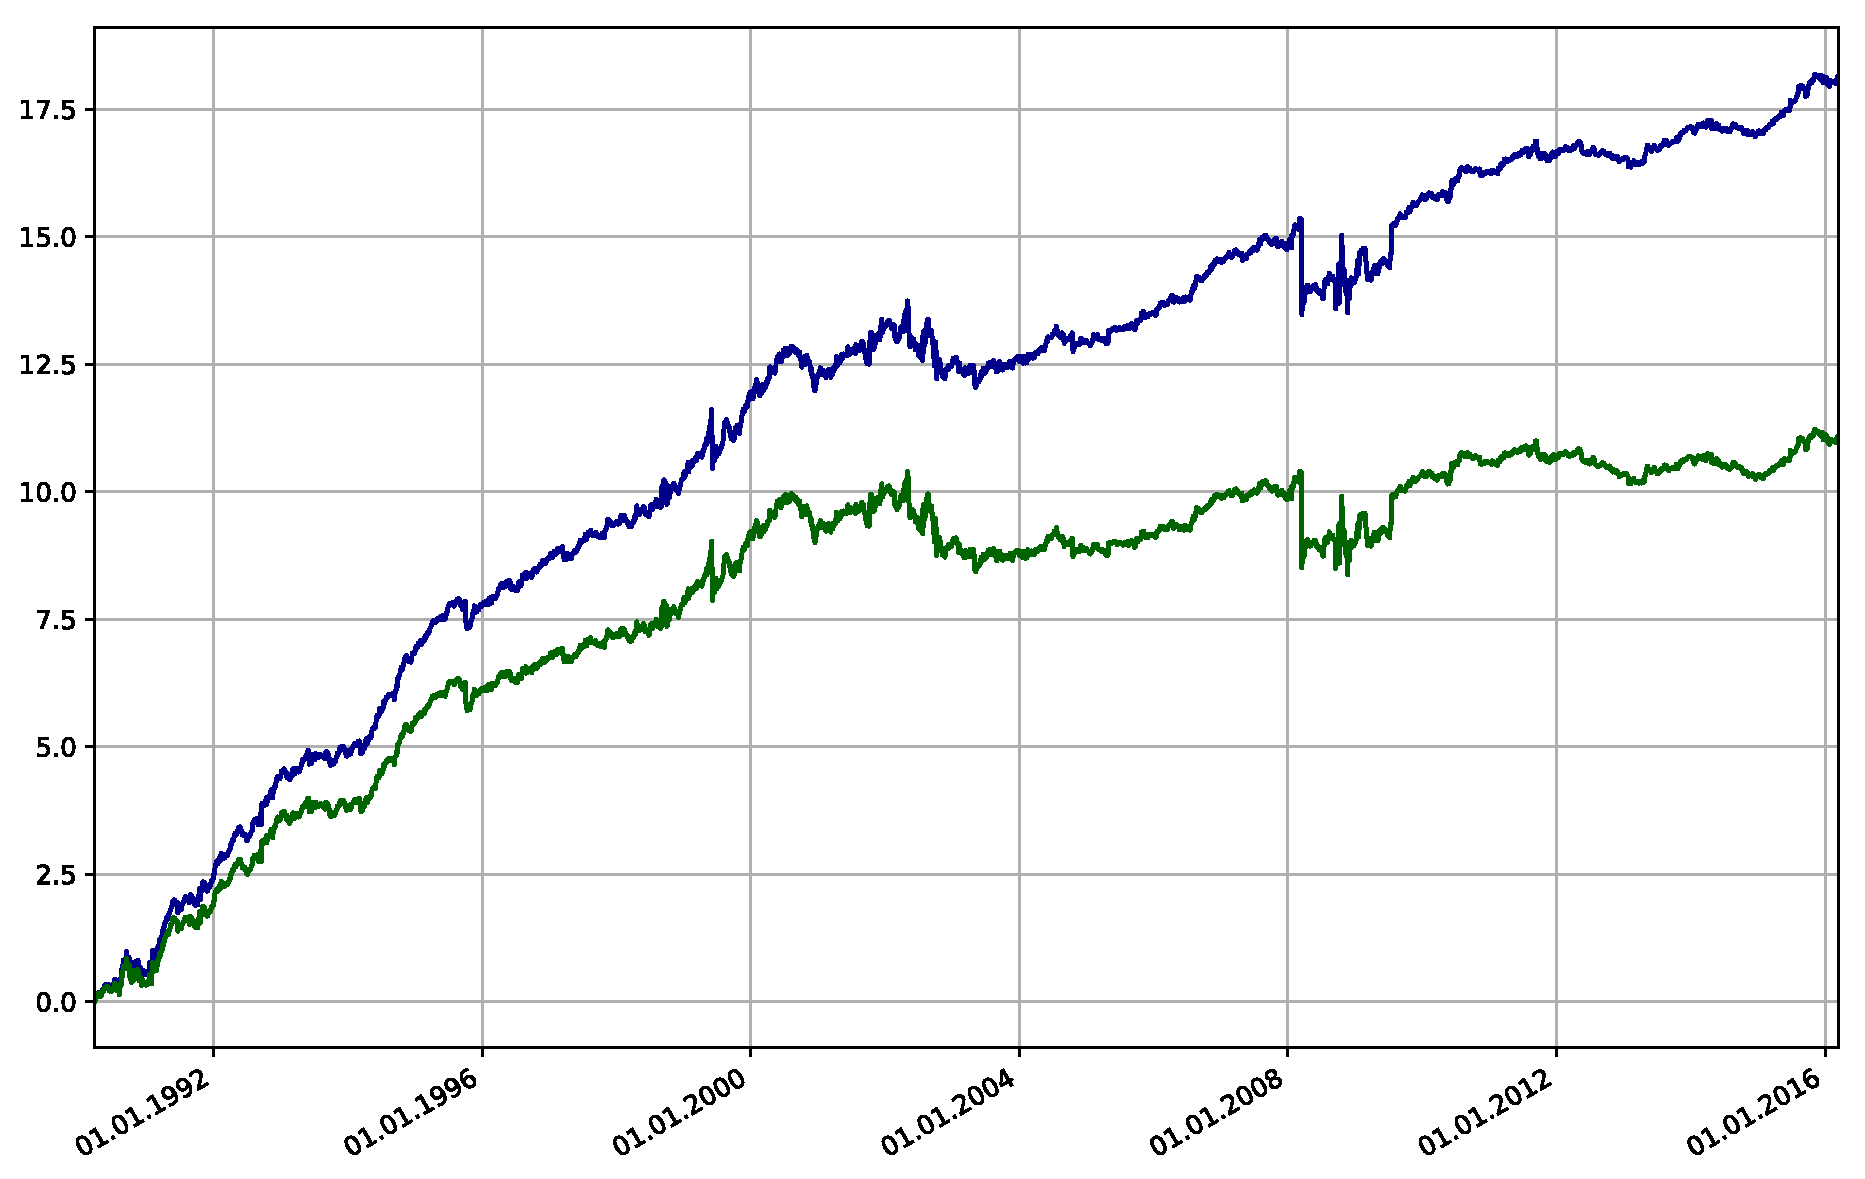
\includegraphics[width=\textwidth]{graphics/sp500full-profits.pdf}
%        \caption*{Simulation results on all assets from S\&P 500 index.}
%    \end{figure}}
%    \only<2>{
%      \begin{table}
%        \centering
%        \caption*{Simulation results on all assets from S\&P 500 index.}
%        \resizebox{0.8\textwidth}{!}{\begin{tabular}{lr}
%            \toprule
%            Results: & \\
%            \midrule
%            \textbf{without transaction costs:} & \\
%            \hspace{.5em}total profit & 18.09261 \\
%            \hspace{.5em}Sharpe ratio & 0.87507 \\
%            \midrule
%            \textbf{including transaction costs of 0.10\%:} & \\
%            \hspace{.5em}total profit & 11.03961 \\
%            \hspace{.5em}Sharpe ratio & 0.53382 \\
%            \midrule
%            average turnover rate  & 1.04088 \\
%            average consistency & 0.55817 \\
%            average precision & 0.52642 \\
%            \bottomrule
%        \end{tabular}}
%    \end{table}}
%  \end{frame}

  \section{Conclusion}
  {
  \setbeamertemplate{footline}{
  	\begin{center}
	  	\tiny{This work has been supported in part by the Croatian Science Foundation under the project 5349.} \\
  		
\includegraphics[height=0.5cm]{graphics/HRZZ.jpg}
    \end{center}
  }
  \begin{frame}
    \frametitle{Conclusion}
    \begin{itemize}
      \item \textbf{enhancement} of present methods of statistical arbitrage
      \item algorithm performs \textbf{better} when there is \textbf{more} assets available, allows for portfolio diversification
      \item algorithm works \textbf{well} even if \emph{short position} is not allowed
%      \item algorithm doesn't take \textbf{systemic risk} into account
    \end{itemize}
    
  \end{frame}
  }
\end{document}